\documentclass[11pt,compress,t,notes=noshow, xcolor=table]{beamer}
\usepackage[]{graphicx}\usepackage[]{color}
% maxwidth is the original width if it is less than linewidth
% otherwise use linewidth (to make sure the graphics do not exceed the margin)
\makeatletter
\def\maxwidth{ %
  \ifdim\Gin@nat@width>\linewidth
    \linewidth
  \else
    \Gin@nat@width
  \fi
}
\makeatother

\definecolor{fgcolor}{rgb}{0.345, 0.345, 0.345}
\newcommand{\hlnum}[1]{\textcolor[rgb]{0.686,0.059,0.569}{#1}}%
\newcommand{\hlstr}[1]{\textcolor[rgb]{0.192,0.494,0.8}{#1}}%
\newcommand{\hlcom}[1]{\textcolor[rgb]{0.678,0.584,0.686}{\textit{#1}}}%
\newcommand{\hlopt}[1]{\textcolor[rgb]{0,0,0}{#1}}%
\newcommand{\hlstd}[1]{\textcolor[rgb]{0.345,0.345,0.345}{#1}}%
\newcommand{\hlkwa}[1]{\textcolor[rgb]{0.161,0.373,0.58}{\textbf{#1}}}%
\newcommand{\hlkwb}[1]{\textcolor[rgb]{0.69,0.353,0.396}{#1}}%
\newcommand{\hlkwc}[1]{\textcolor[rgb]{0.333,0.667,0.333}{#1}}%
\newcommand{\hlkwd}[1]{\textcolor[rgb]{0.737,0.353,0.396}{\textbf{#1}}}%
\let\hlipl\hlkwb

\usepackage{framed}
\makeatletter
\newenvironment{kframe}{%
 \def\at@end@of@kframe{}%
 \ifinner\ifhmode%
  \def\at@end@of@kframe{\end{minipage}}%
  \begin{minipage}{\columnwidth}%
 \fi\fi%
 \def\FrameCommand##1{\hskip\@totalleftmargin \hskip-\fboxsep
 \colorbox{shadecolor}{##1}\hskip-\fboxsep
     % There is no \\@totalrightmargin, so:
     \hskip-\linewidth \hskip-\@totalleftmargin \hskip\columnwidth}%
 \MakeFramed {\advance\hsize-\width
   \@totalleftmargin\z@ \linewidth\hsize
   \@setminipage}}%
 {\par\unskip\endMakeFramed%
 \at@end@of@kframe}
\makeatother

\definecolor{shadecolor}{rgb}{.97, .97, .97}
\definecolor{messagecolor}{rgb}{0, 0, 0}
\definecolor{warningcolor}{rgb}{1, 0, 1}
\definecolor{errorcolor}{rgb}{1, 0, 0}
\newenvironment{knitrout}{}{} % an empty environment to be redefined in TeX

\usepackage{alltt}
\newcommand{\SweaveOpts}[1]{}  % do not interfere with LaTeX
\newcommand{\SweaveInput}[1]{} % because they are not real TeX commands
\newcommand{\Sexpr}[1]{}       % will only be parsed by R
\newcommand{\xmark}{\ding{55}}%


\usepackage[english]{babel}
\usepackage[utf8]{inputenc}

\usepackage{dsfont}
\usepackage{verbatim}
\usepackage{amsmath}
\usepackage{amsfonts}
\usepackage{amssymb}
\usepackage{bm}
\usepackage{csquotes}
\usepackage{multirow}
\usepackage{longtable}
\usepackage{booktabs}
\usepackage{enumerate}
\usepackage[absolute,overlay]{textpos}
\usepackage{psfrag}
\usepackage{algorithm}
\usepackage{algpseudocode}
\usepackage{eqnarray}
\usepackage{arydshln}
\usepackage{tabularx}
\usepackage{placeins}
\usepackage{tikz}
\usepackage{setspace}
\usepackage{colortbl}
\usepackage{mathtools}
\usepackage{wrapfig}
\usepackage{bm}
\usepackage{amsmath}
\usepackage{pifont}
\usepackage{xcolor} %colored math symbols

\usetikzlibrary{shapes,arrows,automata,positioning,calc,chains,trees, shadows}
\tikzset{
  %Define standard arrow tip
  >=stealth',
  %Define style for boxes
  punkt/.style={
    rectangle,
    rounded corners,
    draw=black, very thick,
    text width=6.5em,
    minimum height=2em,
    text centered},
  % Define arrow style
  pil/.style={
    ->,
    thick,
    shorten <=2pt,
    shorten >=2pt,}
}

\usepackage{subfig}

% Defines macros and environments
\usepackage{../../style/lmu-lecture}


\let\code=\texttt
\let\proglang=\textsf

\setkeys{Gin}{width=0.9\textwidth}

\setbeamertemplate{frametitle}{\expandafter\uppercase\expandafter\insertframetitle}

\usepackage{bbm}
% basic latex stuff
\newcommand{\pkg}[1]{{\fontseries{b}\selectfont #1}} %fontstyle for R packages
\newcommand{\lz}{\vspace{0.5cm}} %vertical space
\newcommand{\dlz}{\vspace{1cm}} %double vertical space
\newcommand{\oneliner}[1] % Oneliner for important statements
{\begin{block}{}\begin{center}\begin{Large}#1\end{Large}\end{center}\end{block}}


%new environments
\newenvironment{vbframe}  %frame with breaks and verbatim
{
 \begin{frame}[containsverbatim,allowframebreaks]
}
{
\end{frame}
}

\newenvironment{vframe}  %frame with verbatim without breaks (to avoid numbering one slided frames)
{
 \begin{frame}[containsverbatim]
}
{
\end{frame}
}

\newenvironment{blocki}[1]   % itemize block
{
 \begin{block}{#1}\begin{itemize}
}
{
\end{itemize}\end{block}
}

\newenvironment{fragileframe}[2]{  %fragile frame with framebreaks
\begin{frame}[allowframebreaks, fragile, environment = fragileframe]
\frametitle{#1}
#2}
{\end{frame}}


\newcommand{\myframe}[2]{  %short for frame with framebreaks
\begin{frame}[allowframebreaks]
\frametitle{#1}
#2
\end{frame}}

\newcommand{\remark}[1]{
  \textbf{Remark:} #1
}


\newenvironment{deleteframe}
{
\begingroup
\usebackgroundtemplate{
\includegraphics[width=\paperwidth,height=\paperheight]{../style/color/red.png}}
 \begin{frame}
}
{
\end{frame}
\endgroup
}
\newenvironment{simplifyframe}
{
\begingroup
\usebackgroundtemplate{
\includegraphics[width=\paperwidth,height=\paperheight]{../style/color/yellow.png}}
 \begin{frame}
}
{
\end{frame}
\endgroup
}\newenvironment{draftframe}
{
\begingroup
\usebackgroundtemplate{
\includegraphics[width=\paperwidth,height=\paperheight]{../style/color/green.jpg}}
 \begin{frame}
}
{
\end{frame}
\endgroup
}
% https://tex.stackexchange.com/a/261480: textcolor that works in mathmode
\makeatletter
\renewcommand*{\@textcolor}[3]{%
  \protect\leavevmode
  \begingroup
    \color#1{#2}#3%
  \endgroup
}
\makeatother


\input{../../latex-math/basic-math}
\input{../../latex-math/basic-ml}
\input{../../latex-math/ml-nn}

\title{Deep Learning}

\date{}

\begin{document}
\newcommand{\titlefigure}{plots/fgsm_mod.png}
%modify picture
\newcommand{\learninggoals}{
  \item Advanced adversarial training 
  \item Projected gradient descent
  \item Fast gradient sign method
  %\item Principal component analysis
}

\lecturechapter{Adversarial Training Advances}
\lecture{I2DL}


\newcommand{\Dsubtrain}{\mathcal{D}_{\text{subtrain}}}
\newcommand{\Dval}{\mathcal{D}_{\text{val}}}


%%%%%%%%%%%%%%%%%%%%%%%%%%%%%%%%%%%%%%%%%%%%%%%%%%%%%%%%%%%%%%%%%%
% \section{Neural Networks}
%%%%%%%%%%%%%%%%%%%%%%%%%%%%%%%%%%%%%%%%%%%%%%%%%%%%%%%%%%%%%%%%%%



 \begin{vbframe}{Projected Gradient Descent}
    \begin{itemize}
       \item In contrast to logistic regression, neural networks can have a bumpier, 
       non-convex loss surface.     
       \item As a consequence, Danskin's theorem does not longer hold and the inner optimization problem must be solved approximately. 
       \item One approximation method is projected gradient descent (PGD)$^1$.
        \item Let $\fh$ be the pretrained model, $\xv$ the input to the model, $y$ the target and $L\left(y, \fh(\xv | \thetab) \right)$ the loss function used to train the network.
        \item In each gradient descent step, the basic PGD algorithm updates $\deltab$ as: 
        \begin{equation*}
            \deltab^{[t+1]} = \mathcal{P}\left(\deltab^{[t]} + \alpha \nabla_{\deltab} L\left(y, \fh(\xv + \deltab^{[t]}| \thetab) \right) \right)
        \end{equation*}
        where $\mathcal{P}$ denotes the projection onto the ball of interest. \\
        \lz
        {\scriptsize $^1$ Technically speaking, it is gradient \textit{ascent} since we are maximizing a function, but for the sake of generality, we just refer to the process here as gradient descent.}


        %%%%%%%%%%%%%% Original %%%%%%%%%%%%%%%%%%%5
        % \item In essence, we move with a step size $\alpha$ \textbf{in the direction} of the gradient of the loss with respect to $\deltab$. Then we clip the corresponding values of $\deltab$ back to the chosen perturbation set.  
        % \item In case of $\Delta$ being $\mathcal{B}^{\infty}_{\epsilon}$ the projection is
        % \begin{equation*}
        %     \mathcal{P}_{\Delta}(\deltab) = clip(\deltab, [-\epsilon, \epsilon])
        % \end{equation*}
        % \item One gradient step is then defined as 
        % \begin{equation*}
        %     \deltab^{[t+1]} = clip\left(\delta^{[t]}+ \alpha \nabla_{\deltab} L\left(y, \fh(\xv | \thetab) \right), [-\epsilon, \epsilon]\right)
        % \end{equation*}
        %%%%%%%%%%%%%%%%%%%%%%%%%%%%%%%%%%%%%%%%%%%%%%
        
        
        
        \item In essence, $\deltab^{[t+1]}$ is obtained by moving from $\deltab^{[t]}$ (with a step size $\alpha$) \textbf{in the direction} of the gradient of the loss with respect to $\deltab$ (evaluated at $\deltab^{[t]}$) and then projecting back to $\Delta$.
        \item In case where the feasible set is $\mathcal{B}^{\infty}_{\epsilon}$, the projection of an arbitrary vector $\hidz$ is simply:
        \begin{equation*}
            \mathcal{P}(\hidz) = clip(\hidz, [-\epsilon, \epsilon])
        \end{equation*}
        \item Therefore, when $\Delta$ is $\mathcal{B}^{\infty}_{\epsilon}$, one gradient step is then defined as: 
        \begin{equation*}
            \deltab^{[t+1]} = clip\left(\deltab^{[t]}+ \alpha \nabla_{\deltab} L\left(y, \fh(\xv + \deltab^{[t]}| \thetab) \right), [-\epsilon, \epsilon]\right)
        \end{equation*}
        \end{itemize}
        \vspace{-0.5cm}
          \begin{figure}
    \centering
      %\captionsetup{font=footnotesize,labelfont=footnotesize, labelfont = bf}
      \scalebox{0.85}{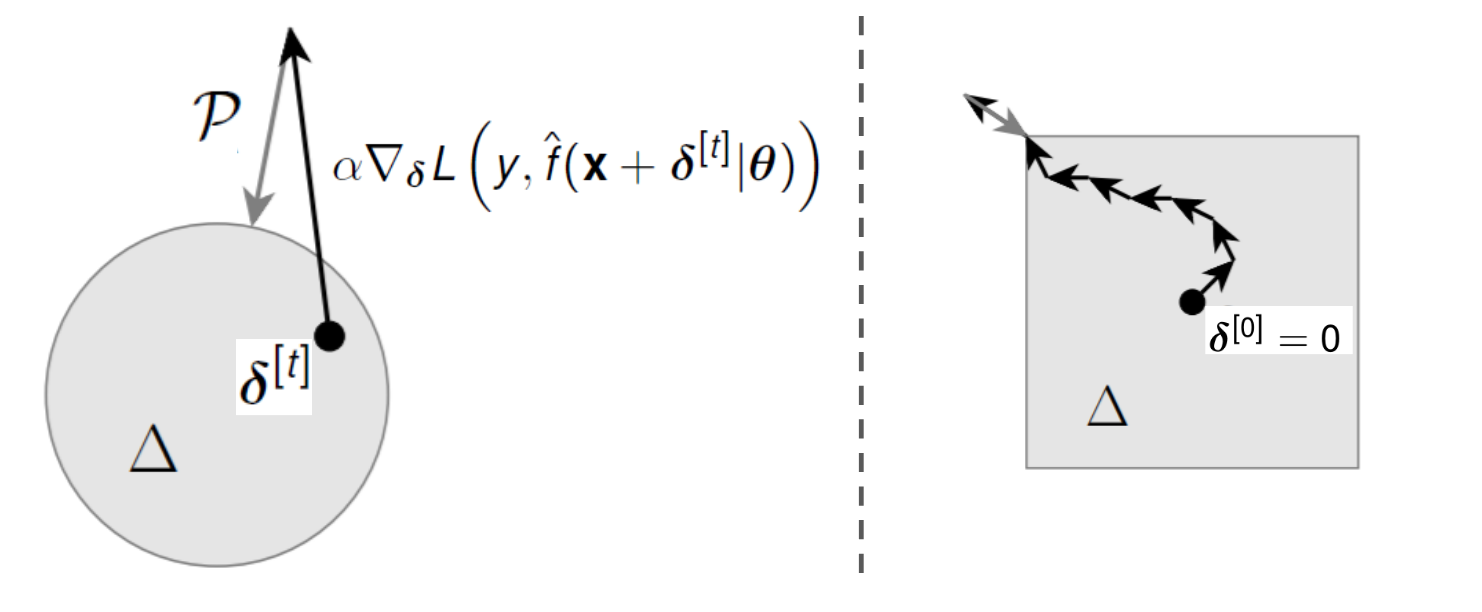
\includegraphics{plots/pgd_mod.png}}
      %\tiny{\\Credit: Kolter and Madry}
      \caption{\small{\textit{Left}: $\deltab^{[t]}+ \alpha \nabla_{\deltab} L(y, \fh(\xv + \deltab^{[t]}| \thetab))$ is projected back to the perturbation set $\Delta$ using $\mathcal{P}$. Here, $\Delta$ is $\mathcal{B}^{2}_{\epsilon}$.
      \textit{Right}: Multiple steps of PGD are shown in case of $\Delta = \mathcal{B}^{\infty}_{\epsilon}$; the projection must be only executed in the last step (Kolter \& Madry, 2019). (Note: A variant of PGD known as \textit{normalized} PGD is shown here. This is why each step has the same size. See Kolter et al. (2019) for details.)}}
  \end{figure}
    
\end{vbframe}
   
     \begin{vbframe} {Fast Gradient Sign Method}
   \begin{itemize}
   \item Fast Gradient Sign Method (FGSM) is a special case of PGD when $\Delta$ = $\mathcal{B}^{\infty}_{\epsilon}$ and $\alpha \rightarrow \infty$ . 
   \item As before, the projection of an arbitrary vector $\hidz$ onto $\mathcal{B}^{\infty}_{\epsilon}$ is $\mathcal{P}(\hidz) = clip(\hidz, [-\epsilon, \epsilon])$. 
   \item As $\alpha \rightarrow \infty$, the elements of $\deltab$ are either set to $-\epsilon$ or $\epsilon$ depending on the sign of the corresponding component of the gradient.
   \item Thus, the FGSM algorithm computes $\deltab$ as
   \small
    \begin{equation*}
      \deltab = \epsilon sign\left(\nabla_{\xv} L\left(y, \fh(\xv | \thetab) \right) \right)
    \end{equation*}
    \normalsize
    \item Note that for FGSM we only conduct one calculation and not multiple gradient descent steps.
    \item Furthermore, because we usually initialize $\deltab^{[0]}$ as $0$     
    \small
    $$\nabla_{\deltab} L\left(y, \fh(\xv + \deltab | \thetab) \right)  = \nabla_{\xv} L\left(y, \fh(\xv | \thetab) \right)$$
    \normalsize
  \begin{figure}
    \centering
      \captionsetup{font=footnotesize,labelfont=footnotesize, labelfont = bf}
      \scalebox{0.32}{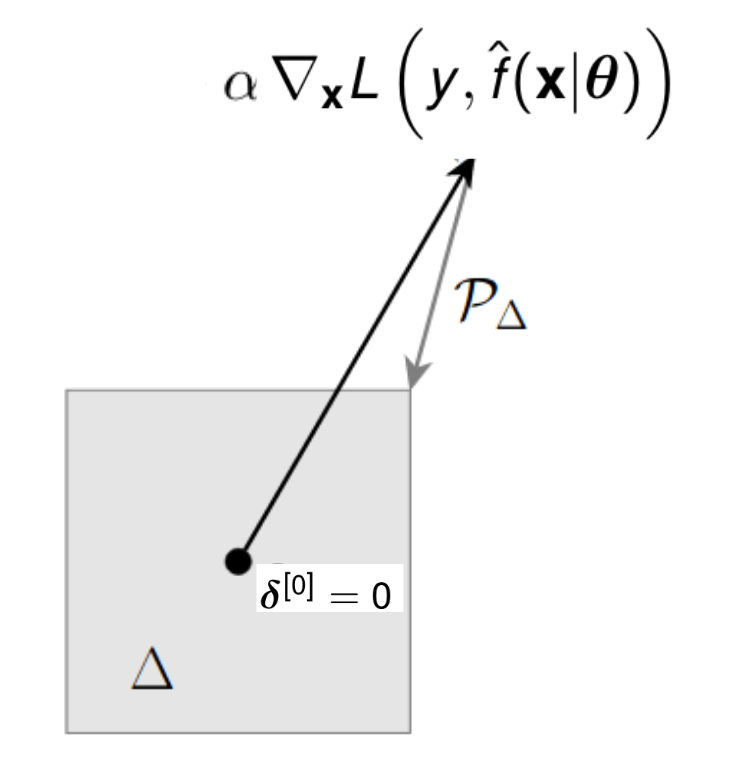
\includegraphics{plots/fgsm_mod.png}}
      %\tiny{\\Credit: Kolter and Madry}
      \caption{$\deltab$ is obtained by setting each element of $\nabla_{\xv} L\left(y, \fh(\xv | \thetab) \right)$ to $-\epsilon$ or $\epsilon$ depending on its sign. Note that this slightly changes the direction of the step that is taken (Kolter \& Madry, 2019).}
  \end{figure}
        \item Implicitly, the (element-wise) $sign$ function is simply a way to constrain the size of the "step" that we take in the direction of the gradient. It is basically equal to a projection of the step back on $\Delta$ (which is $\mathcal{B}^{\infty}_{\epsilon}$).
        \end{itemize}
      \framebreak
        \begin{itemize}
           \item Note: The optimal attack against the linear binary classifier we saw in the last section was also FGSM!
        %\item FGSM assumes that the linear approximation of the function given by its gradient at the point $\xv$ is a reasonably good approximation for the function over the entire region $|\deltab|_{\infty} \le \epsilon$. 
            \end{itemize}
  \begin{figure}
    \centering
      \scalebox{1}{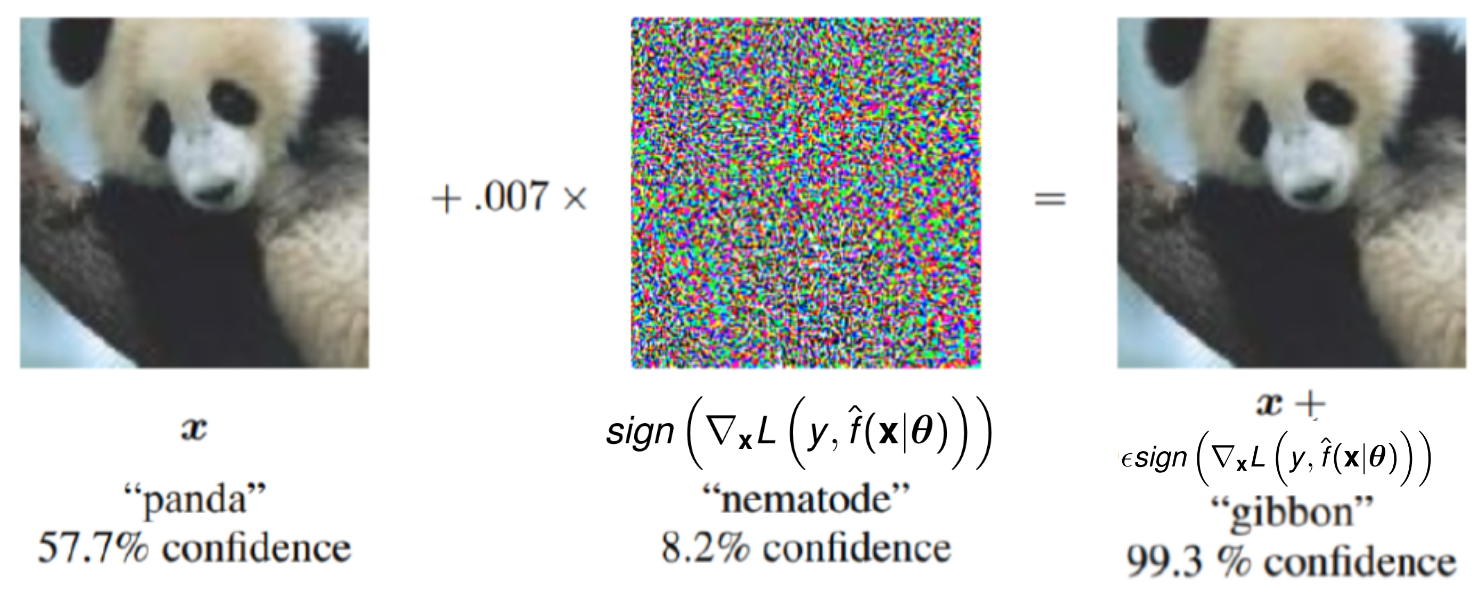
\includegraphics{plots/fgsm_panda.png}}
      %\tiny{\\Credit: Goodfellow}
      \caption{\small{By adding an imperceptibly small vector whose elements are equal to the sign of the elements of the gradient of the cost function with respect to the input, GoogLeNet's classification of the image was changed from 'panda' to 'gibbon'. In this example, the $\epsilon$ is 0.007 (Goodfellow, 2017).}}
  \end{figure}
\end{vbframe}


%%%%%%%%%%%%%%%%%%%%%%%%%%%%%%%%%%%%%%%%%%%%%%%%%%%%%%%%%%%%%%%%%%

%%%%%%%%%%%%%%%%%%%%%%%%%%%%%%%%%%%%%%%%%%%%%%%%%%%%%%%%%%%%%%%%%%
%%%%%%%%%%%%%%%%%%          REFERENCES          %%%%%%%%%%%%%%%%%%
%%%%%%%%%%%%%%%%%%%%%%%%%%%%%%%%%%%%%%%%%%%%%%%%%%%%%%%%%%%%%%%%%%
%\section{References}
\begin{vbframe}
\frametitle{References}
\footnotesize{
\begin{thebibliography}{99}
%%%%%%%%%%%%%%%%%%%%%%%%%%%%%%%%%%
\bibitem[Kolter and Madry (2019)]{1} Zico Kolter and Aleksander Madry (2019)
\newblock Adversarial Robustness - Theory and Practice
\newblock \emph{\url{https://adversarial-ml-tutorial.org/}}
%%%%%%%%%%%%%%%%%%%%%%%%%%%%%%%%%%
\bibitem[Goodfellow et al., 2016]{1} Ian Goodfellow, Yoshua Bengio and Aaron Courville (2016)
\newblock Deep Learning
\newblock \emph{\url{http://www.deeplearningbook.org/}}
%%%%%%%%%%%%%%%%%%%%%%%%%%%%%%%%%%
\bibitem[Goodfellow, 2017]{1} Ian Goodfellow (2017)
\newblock Lecture 16 | Adversarial Examples and Adversarial Training
\newblock \emph{\url{https://www.youtube.com/watch?v=CIfsB_EYsVI}}
%%%%%%%%%%%%%%%%%%%%%%%%%%%%%%%%%%
\bibitem[Goodfellow et al., 2017]{1}  Ian GoodfellowNicolas PapernotSandy HuangRocky DuanPieter AbbeelJack Clark (2017)
\newblock Attacking Machine Learning with Adversarial Examples
\newblock \emph{\url{https://openai.com/blog/adversarial-example-research/}}
%%%%%%%%%%%%%%%%%%%%%%%%%%%%%%%%%%
% \bibitem[Hastie et al., 2009]{2} Trevoe Hastie, Robert Tibshirani and Jerome Friedman (2009)
% \newblock The Elements of Statistical Learning
% \newblock \emph{\url{https://statweb.stanford.edu/\%7Etibs/ElemStatLearn/}}
% %%%%%%%%%%%%%%%%%%%%%%%%%%%%%%%%%%
\bibitem[Nguyen et al., 2015]{1} Anh Nguyen, Jason Yosinski and Jeff Clune (2015)
\newblock Deep Neural Networks are Easily Fooled: High Confidence Predictions for Unrecognizable Images
\newblock \emph{\url{https://arxiv.org/abs/1412.1897}}
%%%%%%%%%%%%%%%%%%%%%%%%%%%%%%%%%%
\bibitem[Krizhevsky et al., 2012]{1} Alex Krizhevsky, Ilya Sutskever and Geoffrey E. Hinto (2012)
\newblock ImageNet Classification with Deep Convolutional Neural Networks. NIPS. 
\newblock \emph{\url{https://papers.nips.cc/paper/4824-imagenet-classification-with-deep-convolutional-neural-networks}}
%%%%%%%%%%%%%%%%%%%%%%%%%%%%%%%%%%
% \bibitem[Hinton et al., 2012]{3} Geoffrey E Hinton, Nitish Srivastava, Alex Krizhevsky Ilya Sutskever and Ruslan Salakhutdinov (2012)
% \newblock Improving neural networks by preventing co-adaptation of feature detectors
% \newblock \emph{\url{http://arxiv.org/abs/1207.0580}}
% %%%%%%%%%%%%%%%%%%%%%%%%%%%%%%%%%%
\bibitem[Maxence Prevost (2018)]{1} Maxence Prevost (2018)
\newblock Adversarial ResNet50 
\newblock \emph{\url{http://arxiv.org/abs/1207.0580}}
%%%%%%%%%%%%%%%%%%%%%%%%%%%%%%%%%%
\bibitem[Sharif et al. (2016)]{1} Mahmood Sharif, Sruti  Bhagavatula and Lujo Bauer (2016)
\newblock Accessorize to a Crime: Real and Stealthy Attacks onState-of-the-Art Face Recognition. Proceedings of the 2016 ACM SIGSAC Conference on Computer and Communications Security.
\newblock \emph{\url{https://dl.acm.org/doi/10.1145/2976749.2978392}}
%%%%%%%%%%%%%%%%%%%%%%%%%%%%%%%%%%
\bibitem[Goodfellow et al., 2014]{5} Goodfellow, Shlens (2014)
\newblock Explaining and Harnessing Adversarial Examples
\newblock \emph{\url{https://github.com/maxpv/maxpv.github.io/blob/master/notebooks/Adversarial_ResNet50.ipynb}}
%%%%%%%%%%%%%%%%%%%%%%%%%%%%%%%%%%
\bibitem[Papernot et al., 2016]{5} Papernot , McDaniel, Goodfellow, Jha, Celik, Swamy (2016)
\newblock Practical Black-Box Attacks against Machine Learning
\newblock \emph{\url{https://arxiv.org/abs/1602.02697}}
%%%%%%%%%%%%%%%%%%%%%%%%%%%%%%%%%%
\bibitem[Athalye et al., 2017]{5} Athalye , Engstrom, Ilyas, Kwok (2017)
\newblock Synthesizing Robust Adversarial Examples
\newblock \emph{\url{https://arxiv.org/abs/1707.07397}}
%%%%%%%%%%%%%%%%%%%%%%%%%%%%%%%%%%
\bibitem[Brown et al., 2018]{1} Tom B. Brown and Catherine Olsson, Research Engineers, Google Brain Team (2018)
\newblock 
Introducing the Unrestricted Adversarial Examples Challenge 
\newblock \emph{\url{https://ai.googleblog.com/2018/09/introducing-unrestricted-adversarial.html}}
%%%%%%%%%%%%%%%%%%%%%%%%%%%%%%%%%%
\end{thebibliography}
}
\end{vbframe}
%%%%%%%%%%%%%%%%%%%%%%%%%%%%%%%%%%%%%%%%%%%%%%%%%%%%%%%%%%%%%%%%%%
%%%%%%%%%%%%%%%%%%%%%%%%%%%%%%%%%%%%%%%%%%%%%%%%%%%%%%%%%%%%%%%%%%
\endlecture
\end{document}
